% !TeX spellcheck = en
\documentclass[review]{elsarticle}

\usepackage{lineno,hyperref}
\usepackage{caption} 
\usepackage{subcaption}
\usepackage{color}

\usepackage{amsmath}
\usepackage{amsthm}
\usepackage{amssymb}
\usepackage{stmaryrd}

\usepackage{array} %Opciones para tablas
\usepackage{graphicx} %Incluir gráficas
\usepackage[justification=centering]{caption}
\usepackage{float}

\usepackage{siunitx}

%\newcommand{\r}{\mathbb{R}}
\def\r{\mathbb{R}}
\def\n{\mathbb{N}}
\def\q{\mathbb{Q}}
\def\z{\mathbb{Z}}
\def\K{\mathbf{K}}

\def\dd{{\rm div}}
\def\gp{{\nabla P}}

\def\trian{\mathcal{T}_h} 
\def\carac{\mathcal{X}}

\def\nn{\textbf{n}}
\def\unn{\textbf{U}}
\def\vnn{\textbf{V}}
\def\vphinn{\boldsymbol{\varphi}}
\def\tnn{\boldsymbol{\tau}}
%\def\sigmnn{\boldsymbol{\sigma}}
\def\bnn{\boldsymbol{\beta}}
\def\x{\mathbf{x}}
\def\esq{\mathcal{E}}

\modulolinenumbers[5]

%\journal{Journal of \LaTeX\ Templates}

%%%%%%%%%%%%%%%%%%%%%%%
%% Elsevier bibliography styles
%%%%%%%%%%%%%%%%%%%%%%%
%% To change the style, put a % in front of the second line of the current style and
%% remove the % from the second line of the style you would like to use.
%%%%%%%%%%%%%%%%%%%%%%%

%% Numbered
%\bibliographystyle{model1-num-names}

%% Numbered without titles
%\bibliographystyle{model1a-num-names}

%% Harvard
%\bibliographystyle{model2-names.bst}\biboptions{authoryear}

%% Vancouver numbered
%\usepackage{numcompress}\bibliographystyle{model3-num-names}

%% Vancouver name/year
%\usepackage{numcompress}\bibliographystyle{model4-names}\biboptions{authoryear}

%% APA style
%\bibliographystyle{model5-names}\biboptions{authoryear}

%% AMA style
%\usepackage{numcompress}\bibliographystyle{model6-num-names}

%% `Elsevier LaTeX' style
\bibliographystyle{elsarticle-num}
%%%%%%%%%%%%%%%%%%%%%%%

\begin{document}


\begin{frontmatter}

\title{An Event Based Representation for Oil Reservoir Simulation using Preconceptual Schemas.}

%% Group authors per affiliation:
%\author{Manuela Bastidas \fnref{myfootnote}}
%\address{Hasselt University, Belgium.}
%\fntext[myfootnote]{Since 1880.}

%% or include affiliations in footnotes:
\author[mymainaddress]{Steven Vel\'asquez-Chanc\'i\corref{mycorrespondingauthor}}
\cortext[mycorrespondingauthor]{Corresponding author}
\ead{svelasquezc@unal.edu.co}
%\ead[url]{www.uhasselt.be/UH/Computational-Mathematics/Members-of-the-research-group.html}

\author[mysecondaryaddress1]{Juan M. Mej\'ia}
\author[mysecondaryaddress2]{ Carlos M. Zapata}

\address[mymainaddress]{National University of Colombia, Medellin. Department of Computer and Decision Science.}
\address[mysecondaryaddress1]{National University of Colombia, Medellin. Department of Processes and Energy.}
\address[mysecondaryaddress2]{National University of Colombia, Medellin. Department of Computer and Decision Science.}


\begin{abstract}
	Oil reservoir simulation is governed by mass conservation laws. In such laws, flow, accumulation, sources and sinks phenomena in porous media are described. Multiple proposals for frameworks and simulations elaboration have been defined. However, those lack concepts and processes tracing, and event representation for physical phenomena. Preconceptual Schema (PS) is used for including the complete structure of an application domain and representing processes emerging in such. Cohesion, consistency, and tracing between concepts and processes is obtained by using PS. In this article, an executable model for Black oil simulation based on a preconceptual schema is proposed. The executable model is validated by running a study case. The results are in accordance with data reported in the literature. The proposed executable model allows for tracing consistently the concepts, processes, and events, which are present in Oil reservoir simulation. 
\end{abstract}

\begin{keyword}
	Porous Media\sep Executable Models\sep Preconceptual Schemas\sep Oil Reservoir Simulation\sep Event based Representation.
\end{keyword}

\end{frontmatter}

\linenumbers

\section{Introduction}
Oil Reservoir simulation is an application of flow in porous media. Macroscopic fluid displacement through a porous rock is studied in such application. Those displacements are due to pressure, saturation, capillary and gravitational changes. Such phenomena are described by mass and momentum conservation laws, which are expressed as a coupled system of differential equations.\\

The black oil model (BOM) is vastly used in industrial efforts. Transport of three fluids at standard conditions is considered in this model. In addition, sink and source terms are involved, which are modeled as wells. Analytic solutions of BOM are unfeasible, hence a numerical solution is required. With this purpose, an spatial and temporal discretization is applied to BOM system of differential equations, the resulting algebraic system is solved using Newton-Raphson method.\\

Preconceptual schemas (PS) are intermediate representations which are useful for establishing a common point of understanding between a stakeholder and a software analyst. Furthermore, PS have elements which allow to represent both structure and dynamics of specific application domains. Moreover, Calle and Nore\~na \textbf{{(citar)}}, extended PS notation for usage in scientific software contexts, which have a greater complexity.\\

Mathematical models, such as Black Oil Model (BOM), are representations that appear in every effort for developing a simulator or framework for oil reservoir simulation. In addition, other representations in which, concepts and processes are shown, lack of traceability and event representation. There are proposals in which traceability is considered, but those are implementation-specific. The whole converges in oil reservoir simulators being developed in an empirical manner.\\

Norena, Calle and Zapata, present PS potential for representing different application domains in scientific software contexts. In their representations, cohesion and traceability between concepts is maintained. Additionally, the whole process is traced in the elaborated PS. In this work, we present the development of an event based representation for oil reservoir simulation using Preconceptual Schemas. The developed representation consists of eight principal concepts, three events which process a simulation, and multiple functions in which reusable portions of representation are used within the PS.

This paper is organized as follows: In Section 2 (ref), we present the Black oil model formulation, its solution method, and PS notation. Section 3 (ref) consists of PS representation and the concepts involved. Section 4 presents a study case for validation of the representation proposed and its translation to C++.

\section{Mathematical Model}
In this section, we present an extended version of Black Oil Model (BOM). Black Oil Model is a system of partial differential equations for three phases: oil (o), gas (g), and water (w), based on volumetric conservation laws at atmospheric temperature and pressure. Solving BOM equations, for a spatial domain $\Omega$ and a time domain $\Theta$, requires finding pressure ($P_{f}(\vec{x},t)$) and saturation ($S_{f}(\vec{x},t)$) fields, with $f \in \left\lbrace o,g,w\right\rbrace $, which satisfy the following:

\begin{align*}
\left.
\begin{array}{l}
\frac{\partial}{\partial t} \left[ \phi \left( \frac{S_{o}}{B_{o}} + \frac{R_{v} S_{g}}{B_{g}} \right) \right]
- \nabla \cdot \left( \frac{1}{B_{o}} \vec{u_{o}} + \frac{R_{v}}{B_{g}} \vec{u_{g}} \right) - \tilde{q}_{o}=0  \\
\frac{\partial}{\partial t} \left[ \phi \left( \frac{S_{g}}{B_{g}} + \frac{R_{s} S_{o}}{B_{o}} \right) \right]
- \nabla \cdot \left( \frac{1}{B_{g}} \vec{u_{g}} + \frac{R_{s}}{B_{o}} \vec{u_{o}} \right) - \tilde{q}_{g} = 0\\
\frac{\partial}{\partial t} \left[\phi \left( \frac{S_{w}}{B_{w}} \right) \right] - \nabla \cdot \left( \frac{1}{B_{w}} \vec{u_{w}} \right) - \tilde{q}_{w} = 0
\end{array}
\right \rbrace  \quad \text{in} \quad \Omega\\
\vec{u}_{f} \cdot \vec{n} = 0, \quad \forall f \in \left\lbrace o,g,w\right\rbrace \quad \text{in} \quad \partial \Omega \\
\left.
\begin{array}{l}
P_{f}(\vec{x},t) = P^{0}_{f}(\vec{x})  \\
S_{f}(\vec{x},t) = S^{0}_{f}(\vec{x})\end{array}
\right \rbrace , \quad t=0
\end{align*}

Where $\vec{u_{f}}$ corresponds to multiphasic Darcy velocity, which is stated as follows: 

\begin{align}
	\label{ec:Darcy}
	&\vec{u_{f}} =\frac{\mathbb{K} k_{rf}}{\mu_{f} } \nabla{\Phi_{f}}
\end{align} 

It is worthnoting that:
\begin{equation}
	\begin{aligned}
	B_{f}= F(P_{f}); \quad
	\mu_{f}= F(P_{f}) \quad \forall f \in \left\lbrace o,g,w\right\rbrace  \\
	R_{s} = F(P_{g}); \quad
	R_{v} = F(P_{o}); \qquad\qquad\\
	k_{rg} = F(S_{g}); \quad
	k_{rw} = F(S_{w}); \quad
	k_{ro} = F(S_{g},S_{w}) \\
	\phi \approx \phi^{0}(1+ C_{r}(P_{o}-P_{ref})) \qquad\qquad
	\end{aligned}
\end{equation}

In addition, {\color{green} wells...}

\subsection{Discretization}
An analytic solution for such a model is infeasible, thus a numerical solution is required. Accordingly, a centered finite volume method is used with an implicit scheme for time discretization. Resulting algebraic equations for BOM in a cell $i$ and a time interval $\left[n;n+1 \right] $ are as follows:

\begin{align}
\label{ec:aceiteDiscretizacion}&\underbrace{\frac{|\Omega_{i}|}{\Delta t}\left[ \phi_{i} \left( \frac{S_{o,i}}{B_{o,i}} + \frac{R_{v,i}S_{g,i}}{B_{g,i}}\right)\right]^{n+1}_{n}}_{\text{Accumulation}} + 
\underbrace{\sum_{c \in S}\left[ T^{n+1}_{o,c} \Delta{\Phi_{o,c}^{n+1}} + R_{v,c}T^{n+1}_{g,c} \Delta{\Phi_{g,c}^{n+1}} \right] }_{\text{Flujo - Aceite}} - Q_{o,i}^{n+1} = 0 \\
\label{ec:gasDiscretizacion}&\underbrace{\frac{|\Omega_{i}|}{\Delta t}\left[ \phi_{i} \left( \frac{S_{g,i}}{B_{g,i}} + \frac{R_{s,i}S_{o,i}}{B_{o,i}}\right)\right]^{n+1}_{n}}_{\text{Acumulación - Gas}} + 
\underbrace{\sum_{c \in S}\left[ T^{n+1}_{g,c}\Delta{\Phi_{g,c}^{n+1} + R_{s,c}T^{n+1}_{o,c} \Delta{\Phi_{o,c}^{n+1}}} \right] }_{\text{Flujo - Gas}} - Q_{g,i}^{n+1} = 0 \\
\label{ec:aguaDiscretizacion}&\underbrace{\frac{|\Omega_{i}|}{\Delta t}\left[ \phi_{i} \left( \frac{S_{w,i}}{B_{w,i}}\right)\right]^{n+1}_{n}}_{\text{Acumulación - Agua}}
+ 
\underbrace{\sum_{c \in S}\left[ T^{n+1}_{w,c}\Delta{\Phi_{w,c}^{n+1}} \right]}_{\text{Flujo - Agua}} - Q_{w,i}^{n+1} = 0 
\end{align}
where:
\begin{align*}
&\left[ \phi_{i} \left( \frac{S_{o,i}}{B_{o,i}} + \frac{R_{v,i}S_{g,i}}{B_{g,i}}\right)\right]^{n+1}_{n} = 
\phi^{n+1}_{i} \left( \frac{S_{o,i}^{n+1}}{B_{o,i}^{n+1}} + \frac{R_{v,i}^{n+1}S_{g,i}^{n+1}}{B_{g,i}^{n+1}}\right) - \phi^{n}_{i} \left( \frac{S_{o,i}^{n}}{B_{o,i}^{n}} + \frac{R_{v,i}^{n}S_{g,i}^{n}}{B_{g,i}^{n}}\right),\\
&\left[ \phi_{i} \left( \frac{S_{g,i}}{B_{g,i}} + \frac{R_{s,i}S_{o,i}}{B_{o,i}}\right)\right]^{n+1}_{n} = 
\phi^{n+1}_{i} \left( \frac{S_{g,i}^{n+1}}{B_{g,i}^{n+1}} + \frac{R_{s,i}^{n+1}S_{o,i}^{n+1}}{B_{o,i}^{n+1}}\right) - \phi^{n}_{i} \left( \frac{S_{g,i}^{n}}{B_{g,i}^{n}} + \frac{R_{s,i}^{n}S_{o,i}^{n}}{B_{o,i}^{n}}\right),\\
&\left[ \phi_{i} \left( \frac{S_{w,i}}{B_{w,i}}\right)\right]^{n+1}_{n} = 
\phi^{n+1}_{i} \left( \frac{S_{w,i}^{n+1}}{B_{w,i}^{n+1}}\right) - \phi^{n}_{i} \left( \frac{S_{w,i}^{n}}{B_{w,i}^{n}}\right)
\end{align*}
$T_{f,c}$ stands for transmissivity in a face $c$, connecting a cell $i$, with another cell $j$.
\begin{align}
\label{ec:Transmissibity}& T_{f,c} = \left(\frac{2}{(\Delta l_{i}/A_{c}K_{l,i})+(\Delta l_{j}/A_{c}K_{l,j})}\right)\frac{k_{rf,c}}{\mu_{f,c}B_{f,c}}
\end{align}


%\section{Mathematical Model}
%
%A model of single-phase and incompressible fluid flow through a porous media can be stated as follows: Let $\Omega\subseteq\r^2$ a closed domain with polygonal boundary $\Gamma:= \bar{\Gamma}_D\cup\bar{\Gamma}_N$, where $\Gamma_D$ and $\Gamma_N$ are the Newmann and Dirichlet boundaries respectively. For a given volumetric source ($\dot{f}$), the problem is to find the pressure $P:\Omega \to \r$ of a fluid satisfying:
%\begin{equation} \label{diff1}
%\begin{aligned}
%	- \dd\left( \frac{\mathbb{K}}{\mu}\gp \right)  &= \dot{f} & &\mbox{in } \Omega \\
%	- \frac{\mathbb{K}}{\mu}\gp\cdot\textbf{n} &= g_N & & \mbox{on } \Gamma_N \\
%	P &= g_D 	& & \mbox{on } \Gamma_D 
%\end{aligned}
%\end{equation}
%where $\mathbb{K} \in \left[ L^{\infty}(\Omega)\right]^2$ is the permeability tensor function and $\mu \in \r$ the viscosity of the fluid.
%
%\subsection{Mixed formulation}
%
%To obtain the approximation of the pressure and the velocity fields, we will use a mixed formulation. This formulation will help us to find a coupled numerical scheme.  First, we rewrite problem \eqref{diff1} using the velocity field $\unn= -\frac{\mathbb{K}}{\mu}\gp$ as
%an auxiliary variable as follows:
%\begin{equation} \label{diff2}
%\begin{aligned} 
%\unn			 	&= -\frac{\mathbb{K}}{\mu}\gp & &\mbox{in } \Omega \\
%{\rm div}\ \unn     &= \dot{f}	& & \mbox{in } \Omega\\
%\unn\cdot\textbf{n} &= g_N				& & \mbox{on } \Gamma_N \\
%P &= g_D 	& & \mbox{on } \Gamma_D  \\
%%P(\x,0) &= P_0 	& &\mbox{en } \Omega 
%\end{aligned}
%\end{equation}
%
%Clearly, if the problem \eqref{diff1} has a unique solution then the problem \eqref{diff2} has an unique solution without additional assumptions.
%
%\subsection{Variational formulation}
%Let $q$ and $\vnn$ be scalar and vectorial functions respectively. These functions live in the same vectorial spaces of $P$ and $\unn$.  Multiplying adequately the equations \eqref{diff2} by $q$ and $\vnn$ and integrating over the domain $\Omega$:
%
%\begin{equation}\label{diff3}
%\begin{aligned} 
%\int_{\Omega} \left( \frac{\mathbb{K}}{\mu} \right) ^{-1} \unn \cdot \vnn  - \int_{\Omega}   (\dd\vnn)P +  \int_{\Gamma}(\vnn\cdot\nn)P &= 0,\\
%- \int_{\Omega} \unn\cdot \nabla q 		+
%\int_{\Gamma} ({\unn}\cdot\nn)\,q &= \int_{\Omega} \dot{f}\,q		
%\end{aligned}
%\end{equation}
%
%The solution $(P,\unn)$ of the strong problem \eqref{diff2} satisfies the integral equation \eqref{diff3}, but this integral formulation has less regularity requests \cite{gatica2014simple}.  For this reason, we will focus all efforts to find a pair of functions  $(\unn_h,P_h)$ who approximate the solution of \eqref{diff3}. 
%
%\section{Methodology}
%
%The target of this paper is to approximate the solution of the pressure $P$ and the gradient $\gp$ over the domain $\Omega$ as accurately as possible. For this, a discretization of the domain is needed.
%
%\subsection{Discrete formulation}
%
%Let $\mathcal{T}_h  $ be a regular triangulation of $\bar{\Omega}$. The set of all edges of the triangulation is $\esq_h$, with subsets $\esq_I$ and $\esq_{\Gamma}$ corresponding to the interior and the boundary faces.
%We will find a discontinuous approximations $(\unn_h,P_h)$ to the solution $(\unn,P)$. Furthermore, the approximations of $P$ and $\unn$ over the skeleton $\esq_h$, will be denoted $\hat{P}$ and $\hat{\unn}$ respectively. A geometrical interpretation of these \textit{numerical fluxes} is shown in Figure \ref{fig:P_gorro}.
%
%The HDG formulation requires the following relation between the unknowns \cite{cockburn2010projection}
%\begin{equation}\label{ContinuidadTrazaNormal}
%\hat{\unn}\cdot\nn= \unn_h\cdot\nn + \xi (P_h-\hat{P})
%\end{equation} 
%for some positive penalty function $\xi>0$ defined on $\partial \trian := \sum_{\esq_h} \partial K$ and constant on each face of the triangulation. 
%%The property \eqref{ContinuidadTrazaNormal} is called \textit{Continuity of the normal trace} and guarantees the consistency of the model 
%\begin{figure}[H]
%	\centering
%	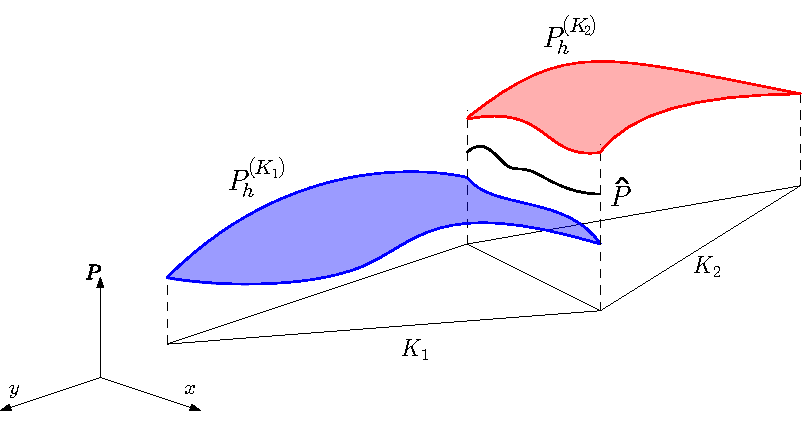
\includegraphics[width=0.8\linewidth]{./Figures/Methodology/P_gorro}
%	\caption{Geometrical interpretation of the numerical flux approximation.}
%	\label{fig:P_gorro}
%\end{figure}
%Over each triangle $K \in \mathcal{T}_h$ the problem \eqref{diff3} can be rewritten as: \textit{To find $(\unn_h,P_h,\hat{P})$ such that:}
%\begin{equation}\label{localp}
%\begin{aligned} 
%\int_K \left( \frac{\mathbb{K}}{\mu} \right) ^{-1} \unn_h \cdot \vnn_h  - \int_K   (\dd\vnn_h)P_h  &= - \int_{\partial K}(\vnn_h\cdot\nn)\hat{P} ,\\
%\int_K   (\dd \unn_h)q_h - \int_{\partial K}\xi\, P_h\,q_h &= 
%\int_{\partial K} \xi\,\hat{P}\,q_h + \int_K \dot{f}\,q_h,		
%\end{aligned}
%\end{equation}
%with $q_h$ and $\vnn_h$ enough regular. Summing over all faces, the normal trace must satisfy
%\begin{equation} \label{normalGlobal1}
%\int_{\partial \trian} \left( \unn_h\cdot\nn + \xi (P_h-\hat{P})\right) \, \mu = \int_{\partial \trian} \tilde{g}_N\mu,
%\end{equation}
%for all $\mu$ defined at $\esq_h$ and where $\tilde{g}_N$ is the extension by zero of $g_N$ over $\esq_h$. The equation \eqref{normalGlobal1} can be called the \textit{Continuity of the normal trace} and guarantees the consistency of the complete scheme. \\
%The set of equations \eqref{localp} is called \textit{Local solver}. Thereby, if we know the solution at edges, reconstruction of the solution $P_h$ and $\unn_h$ is straightforward.
%
%\subsection{Implementation}
%
%For each $K$ and over the edges $e$ in the triangulation $\esq_h$, define the following finite dimensional approximation spaces:
%\begin{equation}\label{spaces}
%\begin{aligned}
%\mathbb{P}_{r_1}(K)   &  = \mathrm{span}\left( \{\psi_j\}_{j=1}^{D_1}\right) , \\
%[\mathbb{P}_{r_2}(K)]^2 & = \mathrm{span}\left( \{\vphinn_j\}_{j=1}^{D_2}\right)  ,  \\
%\mathbb{P}_{r_1}(e) & =  \mathrm{span}\left( \{\phi_j\}_{j=1}^{D_1-1} \right) 
%\end{aligned}
%\end{equation}
%Then we can write $\unn_h$, $P_h$, $\hat{P}$ as lineal combinations of the basis functions \eqref{spaces}. Replacing the finite projections  $\unn_h$, $P_h$ on \eqref{localp} the result is the following \textit{local lineal system}
%
%\begin{align}\label{sistemaEq1}
%\left[\begin{array}{cc}
%\textbf{A}^K & -\textbf{B}^K \\ 
%\textbf{B}^{K^T} & \textbf{C}^K
%\end{array} \right] 
%\left[\begin{array}{c}
%\left[\unn_h \right] \\ 
%\left[ P_h \right]
%\end{array} \right]  = 
%\left[\begin{array}{c}
%- \textbf{D}^K  \\ 
%\textbf{E}^K 
%\end{array} \right] 
%[\hat{P}] + 
%\left[\begin{array}{c}
%\textbf{0}  \\ 
%\textbf{F}^K 
%\end{array} \right],
%\end{align}
%where $\left[\unn_h \right]$ and $\left[ P_h \right]$ denote the degrees of freedom related with the unknowns $\unn_h$ and $P_h$ respectively, and the matrices are given by
%\begin{equation} 
%\begin{aligned} \label{matrices}
%A_{ij}^K &:=  \int_K \left( \frac{\mathbb{K}}{\mu} \right) ^{-1} \vphinn_i \cdot \vphinn_j ,
%& B_{ij}^K &:=   - \int_K   \psi_i \, \dd\vphinn_j ,  \\
%C_{ij}^K &:=\int_{e} \xi\, \psi_i\,\psi_j ,
%& D_{ij}^K &:= \int_{e}(\vphinn_j\cdot\nn)\phi_i,\\  
%E_{ij}^K &:= \int_{e} \xi\,\phi_i\,\psi_j,
%& F_{j}^K  &:=  \int_K f\,\psi_j.
%\end{aligned}
%\end{equation}
%Then, we can rewrite the local linear system \eqref{sistemaEq1} in a compact form as 
%
%\begin{equation}\label{sistemaEq}
%\begin{aligned}
%\left[ \textbf{M}^K  \right] 
%\left[\begin{array}{c}
%\left[\unn_h\right] \\ 
%\left[ P_h \right]
%\end{array} \right]  = 
%\left[\begin{array}{c}
%- \textbf{D}^K  \\ 
%\textbf{E}^K 
%\end{array} \right] 
%[\hat{P}] + 
%\left[\begin{array}{c}
%\textbf{0}  \\ 
%\textbf{F}^K 
%\end{array} \right].
%\end{aligned}
%\end{equation}
%
%Imposing the normal trace continuity condition over the edges \eqref{normalGlobal1}, we obtain the \textit{global lineal system} 
%\begin{align}\label{globalsis1}
%\sum_{K \in \trian} \int_{\partial K} (\hat{\unn}\cdot \nn_K ) \phi_j   &=  \sum_{K \in \trian}  \int_{\partial K} \unn_h \cdot \nn_K - \xi(P_h-\hat{P})\phi_j  \nonumber  \\
%&= \left[\begin{array}{c}
%\textbf{D}^K  \\ 
%\textbf{E}^K 
%\end{array} \right] \left[\begin{array}{c}
%\left[\unn_h\right] \\ 
%\left[ P_h \right]
%\end{array} \right] -  \textbf{R}^K [\hat{P}], 
%\end{align}
%where $\textbf{R}^K$ is a local matrix $ R_{ij}^K := \int_{e} \xi\,\phi_i\,\phi_j $. Replacing  \eqref{sistemaEq} in \eqref{globalsis1} and summing over all $\esq_h$:
%
%\begin{equation*}
%\int_{\esq_h} (g_N\,\mathbb{I}_{\esq_{\Gamma}}\cdot\nn)\phi_j = \sum_{K \in \trian} \textbf{X}^K[\hat{P}] + \textbf{Y}^K,
%\end{equation*}
%
%where 
%\begin{align*}
%\textbf{X}^K &= \left[\begin{array}{c}
%\textbf{D}^K \\ \textbf{E}^K
%\end{array} \right]^T 
%\textbf{M}^{K^{-1}}\left[\begin{array}{c}
%-\textbf{D}^K  \\ 
%\textbf{E}^K 
%\end{array} \right] - \textbf{R}^K 
%\end{align*}
%and
%\begin{align*}
%\textbf{Y}^K &= \left[\begin{array}{c}
%\textbf{D}^K \\ \textbf{E}^K
%\end{array} \right]^T   \textbf{M}^{K^{-1}} 
%\left[\begin{array}{c}
%\textbf{0}  \\ 
%\textbf{F}^K 
%\end{array} \right].
%\end{align*}
%
%Finally, the global system is
%\begin{equation}\label{sistemaEqhdg2}
%\textbf{H}[\hat{P}] = \textbf{G}_N + \textbf{K} 
%\end{equation}
%where $\textbf{G}_N$ is the null vector except for the positions related to the Newmann boundary. And $\textbf{H}$ and $\textbf{K}$ are the assembly of  $\textbf{X}^K$ and $\textbf{Y}^K$ respectively. 
%
%\section{Numerical examples}
%
%In this section, we will address three examples. We will use the SI units in these equations: $\dot{f}$ in units of volumetric flux, the natural unit of $\mathbb{K}$ is  $\mathrm{m^2}$, $\mu$ in $\mathrm{Pa}\cdot\mathrm{s}$ and  pressure in $\mathrm{Pa}$. 
%
%\subsection{Laplace equation}
%Initially we will validate the HDG method with the Laplacian equation in a two dimensional square with Dirichlet boundary condition ($\Gamma_D$) except for the north face where the boundary condition is Neumann ($\Gamma_N$) as is shown in Figure \ref{fig:cuadrito}.  The flow is assumed to be incompressible, steady-state, Newtonian and the porous medium is isotropic \cite{lynd2016application} 
%\begin{equation} 
%\label{laplace}
%\begin{aligned} 
%- \dd\left( \gp \right)  &= 0 & &\mbox{in } \Omega, \\
%- \frac{\partial P}{\partial y} &= \frac{1}{10}\sin\left( \frac{\pi x}{800}\right) & & \mbox{on } \Gamma_N,\\
%P &= 0 	& & \mbox{on } \Gamma_D. 
%\end{aligned}
%\end{equation}
%The analytic solution of the problem \eqref{laplace} is given by
%\begin{equation}
%P(x,y) = \frac{80}{\pi \cosh(\pi)} \sin\left( \frac{\pi x}{800}\right) \sinh\left( \frac{\pi y}{800}\right).
%\end{equation}
%\begin{figure}[H]
%	\centering
%	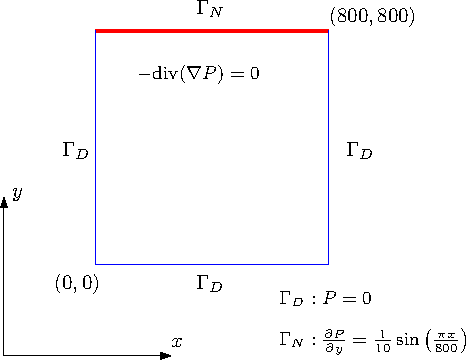
\includegraphics[width=0.6\linewidth]{./Figures/Examples/Laplacian/laplacianProblem.pdf}
%	\caption{Geometry and boundary conditions of the Laplace equation example.}
%	\label{fig:cuadrito}
%\end{figure}
%
%Figure \ref{fig:soltexas} shows the numerical solution of this problem and the  magnitude of the pressure gradient.
%\begin{figure}[H]
%	\centering
%	\begin{subfigure}[b]{0.45\textwidth}
%		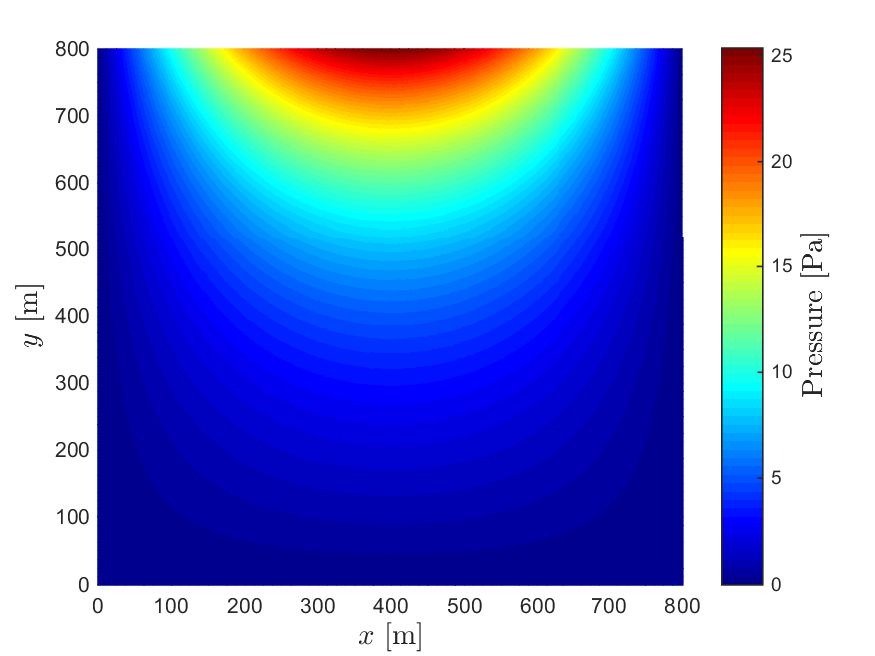
\includegraphics[width=\textwidth]{./Figures/Examples/Laplacian/soltexas1}
%		\caption{Pressure field.}
%		\label{fig:soltexas1}
%	\end{subfigure}
%	\begin{subfigure}[b]{0.45\textwidth}
%		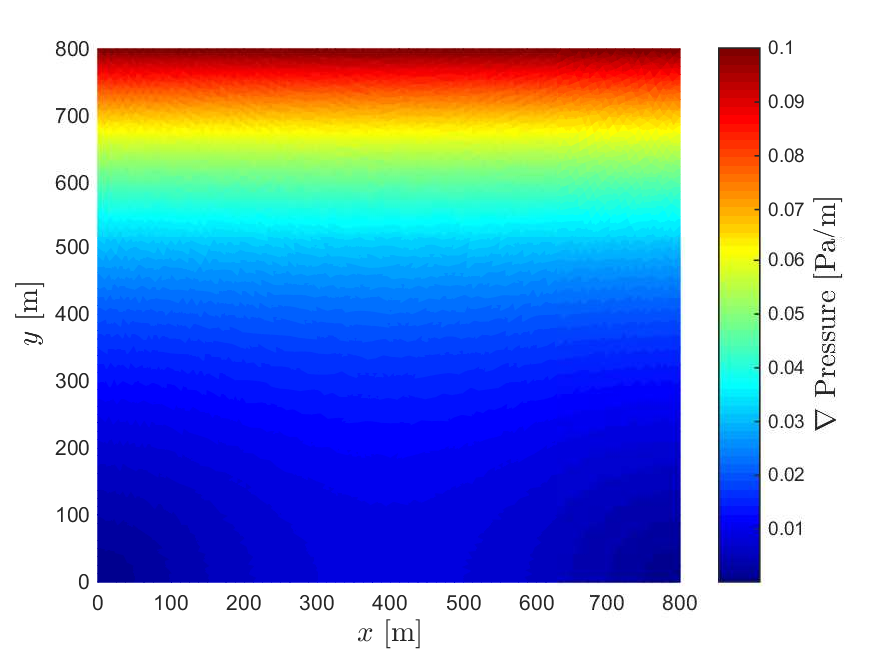
\includegraphics[width=\textwidth]{./Figures/Examples/Laplacian/soltexas1gp}
%		\caption{Gradient magnitude.}
%		\label{fig:soltexas1gp}
%	\end{subfigure}
%	\caption{Numerical solution of the Laplace equation for isotropic case using a mesh with $10784$ elements}
%	\label{fig:soltexas}
%\end{figure}
%
%To analyze the behavior of the flow the streamlined plot is presented in Figure \ref{fig:soltexas1st}. 	This result indicates that the particles will travel from high to low potentials, being consistent with the equation \eqref{diff2}.
%
%\begin{figure}[H]
%	\centering
%	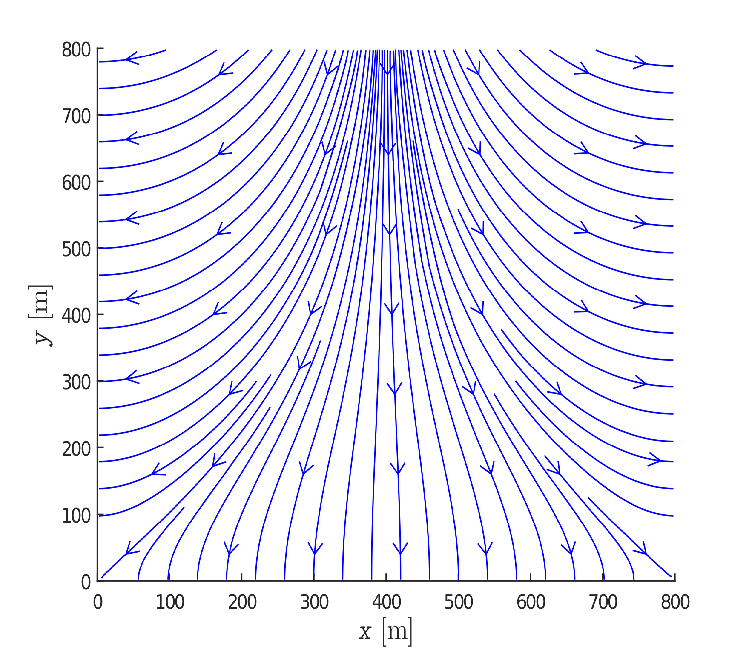
\includegraphics[width=0.6\linewidth]{./Figures/Examples/Laplacian/soltexas1stream_rem}
%	\caption[Test geometry 1]{Streamlines of the Laplace example.}
%	\label{fig:soltexas1st}
%\end{figure}
%
%The accuracy of the method is computed based on the relative error of the numerical solution using the $L^2$-norm, i.e $\frac{\|P-P_h\|_2}{\|P\|_2}$.
%
%%\begin{equation}
%% =  \frac{ \left( \int_{\Omega} \left( P-P_h\right)^2 \right) ^{1/2}}{ \left( \int_{\Omega}  P^2 \right) ^{1/2}}.
%%\end{equation}
%
%The convergence of the relative error is presented in Table \ref{errorL2Texas1}., in terms of the number elements and degrees of freedom (dof) for five different mesh sizes. 
%
%\begin{table}[H]
%	\begin{center}
%		\begin{tabular}{|c||c|c|}
%			\hline
%			nElement & d.o.f &  Error \\ \hline\hline
%			40       &360    & 0.10200\\
%			184      &1656   & 0.02016\\
%			676      &6084   & 0.00532\\
%			2656     &23904  & 0.00129\\
%			10784    &97056  & 0.00029\\ \hline	
%		\end{tabular}
%		\caption{Convergence of the error with the $L^2$-norm.}\label{errorL2Texas1}
%	\end{center}
%\end{table}
%The error analysis presented in Table \ref{errorL2Texas1} indicates that the HDG method is enough accurate and the numerical solution converges to the analytical solution when the mesh is refined.
%
%Now, we will solve the same flow problem in an anisotropic medium with a different permeability tensor
%\begin{align}\label{Kpermtexas}
%\mathbb{K} = \left[\begin{array}{cc}
%10^{-10} \, \mathrm{m^2} & 0 \\ 
%0 & 1 \, \mathrm{m^2}
%\end{array} \right] 
%\end{align}
%and viscosity $\mu = 10^{-3}$ $\mathrm{Pa}\cdot\mathrm{s}$. The Figure \ref{fig:soltexas2} presents the numerical solution of this problem using the HDG method.
%
%\begin{figure}[H]
%	\centering
%	\begin{subfigure}[b]{0.45\textwidth}
%		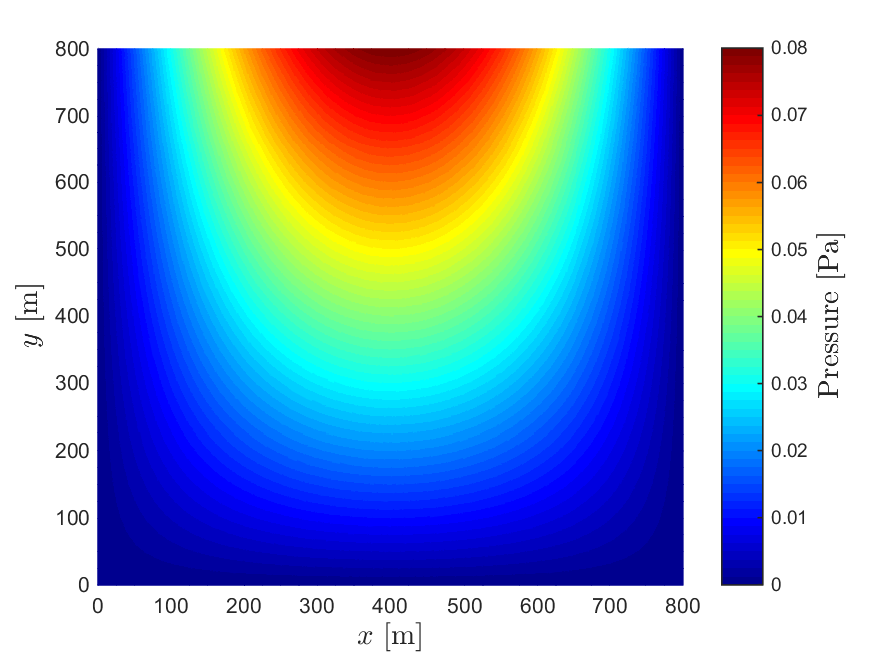
\includegraphics[width=\textwidth]{./Figures/Examples/Laplacian_Anisotorpy/soltexas2.pdf}
%		\caption{Pressure field.}
%		\label{fig:soltexas2p}
%	\end{subfigure}
%	\begin{subfigure}[b]{0.45\textwidth}
%		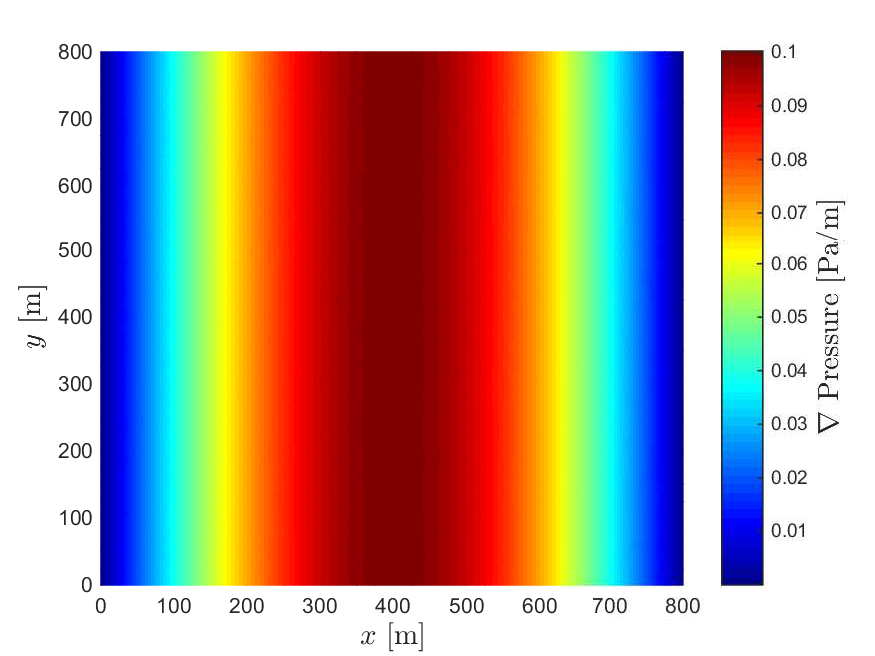
\includegraphics[width=\textwidth]{./Figures/Examples/Laplacian_Anisotorpy/soltexas2gp.pdf}
%		\caption{Gradient of the pressure.}
%		\label{fig:soltexas2gp}
%	\end{subfigure}
%	\caption{Numerical solution of the Laplace equation for the anisotropic case using a mesh with $10784$ elements.}
%	\label{fig:soltexas2}
%\end{figure}
%
%Figure \ref{fig:soltexas2p} shows the pressure field in the anisotropic case, it is sharper than the isotropic one, although, the boundary conditions are the same in both cases. The source in the top boundary creates a preferential flow through in the $y$-direction. It is indicated by the high pressure gradient in the central area of Figure \ref{fig:soltexas2gp}. The above mentioned property can be also observed in  Figure \ref{fig:soltexas2st}, where the corresponding streamlines coincide with the expected behavior, which is the preferential flow direction \cite{FERGUSON1996}. 
%\begin{figure}[H]
%	\centering
%	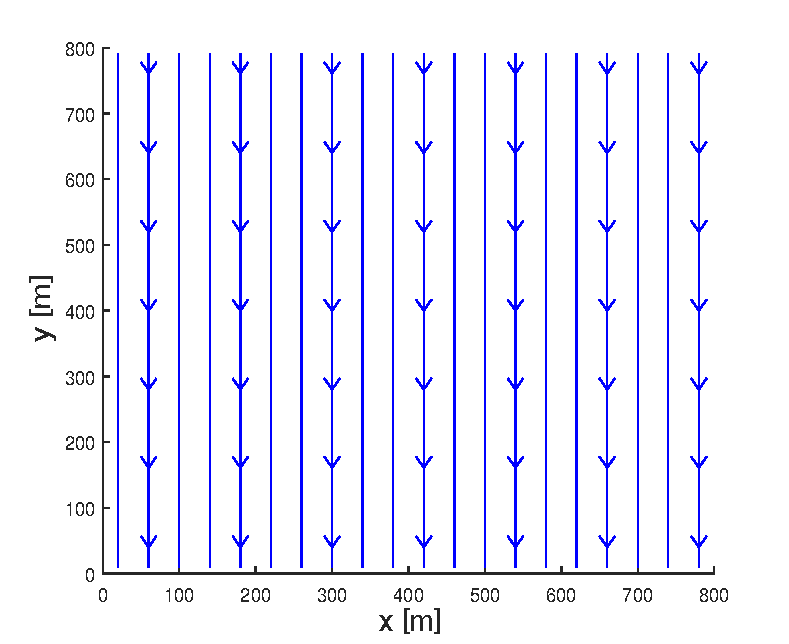
\includegraphics[width=0.45\linewidth]{./Figures/Examples/Laplacian_Anisotorpy/soltexas2stream.pdf}
%	\caption[Test geometry 1]{Streamlines of the anisotropic example.}
%	\label{fig:soltexas2st}
%\end{figure}
%
%The solution in this example shows the HDG advantage over the traditional unstructured FMV, which has problems of convergence when the ratio between the components of the permeability tensor is larger than 1:1000. \cite{FERGUSON1996} That is because the cross diffusion term that appears in cell-centered FVM discretization \cite{jasak1996error}\cite{juretic2005error}   acquires a significant magnitude that affects the global convergence of the method \cite{jayantha2003}\cite{loudyi}.
%  
%\subsection{Five-spots problem}
%The second problem is a classical two-dimensional flow problem: a confined five-spot pattern where each fluid injector and producer point is assumed to act as a point source and sink (negative source) respectively \cite{KATIYAR}.
%
%\subsubsection{Case 1.}
%
% The Figure \ref{fig:5puntos1ex}, displays the geometry of the five-spot problem domain. Here the single phase flow is assumed incompressible, Newtonian, in steady-state and the porous medium is isotropic.  The analytical solution of this problem is given by:
%\begin{equation}
%\label{exact_5spot}
%P(x,y) = -\frac{\mu}{4 \pi K} \sum_{i=1}^5 q_i\ln\left( (x-x_i)^2+ (y-y_i)^2\right) 
%\end{equation}
%where $\mu = 10^{-3}$ $\mathrm{Pa}\cdot\mathrm{s}$, the permeability $K = 10^{-13}$ $\mathrm{m^2}$, and the volumetric flow rate at well $i$: $\dot{q}_i= \pm 10^{-3}$  $\frac{\mathrm{m^3}}{\mathrm{s}}$.
%In order of the symmetry of this problem, we analyze only one quarter of the problem. Then the injector well and the producer will be at coordinates $(x_1,y_1)= (0,0)$ and $(x_2,y_2)= (400,400)$ respectively.   
%
%\begin{figure}[H]
%	\centering
%	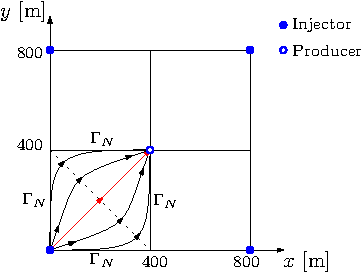
\includegraphics[width=0.5\linewidth]{./Figures/Examples/FiveSpot/fivepointfig.pdf}
%	\caption[Test geometry 1]{Geometry of the five-spot problem.}
%	\label{fig:5puntos1ex}
%\end{figure}
%
%Also, since the sources are punctual in the corners, it is necessary to refine the simulation mesh as shown in the Figure \ref{fig:5puntosMesh}. This is done in order to reproduce numerically the punctual influence of the source, in the matrix $F^k$ in equation \eqref{sistemaEq1}.
%\begin{figure}[H]
%	\centering
%	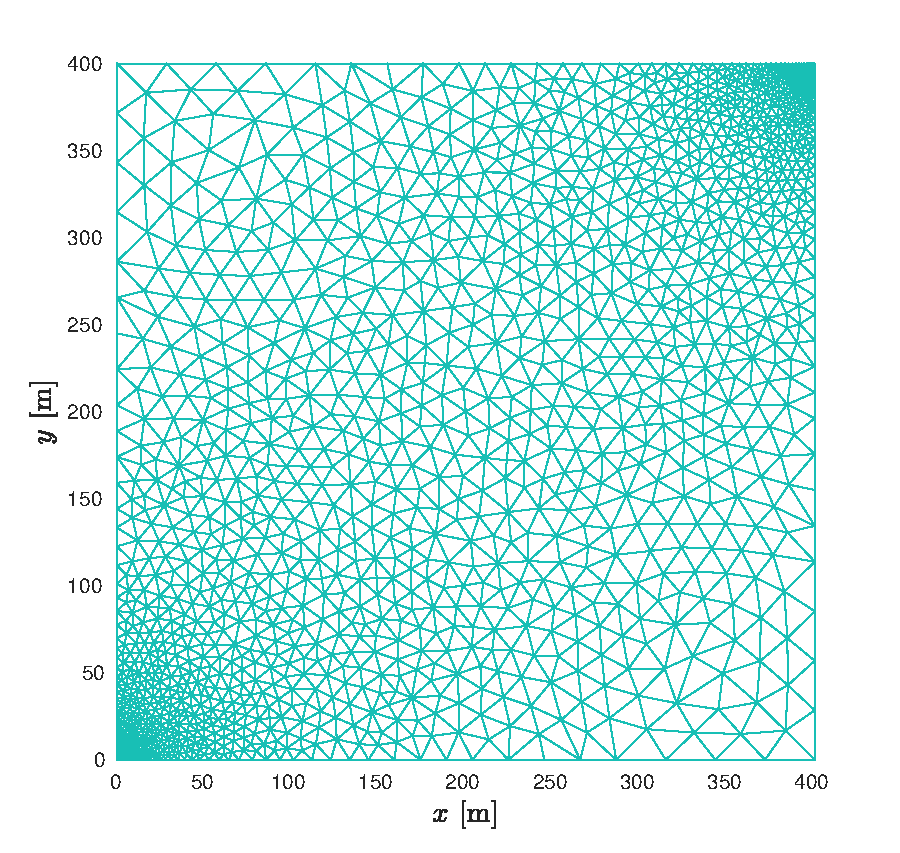
\includegraphics[width=0.6\linewidth]{./Figures/Examples/FiveSpot/5spot1_Mesh.pdf}
%	\caption[Test geometry 1]{Mesh for the simulation.}
%	\label{fig:5puntosMesh}
%\end{figure}
%
%
%The results for this five-spot problem are presented in Figure \ref{fig:fiveResults}. The pressure field (in $\mathrm{MPa}$) is indicated in the Figure \ref{fig:5puntos2}, where a radial variation of the pressure in the neighbor of the wells is observed.  Also, Figures \ref{fig:5puntos1_Diag} and \ref{fig:5puntos1_boundSol} shows the comparative analysis between the analytical solution and the numerical solution along the diagonal of the domain and the $y$-boundaries respectively. Moreover, the comparison of the volumetric flows at the borders is given in Figure \ref{fig:5puntos1_limit}, which are a direct output of the method by directly obtaining the gradients of the solution.
%
%\begin{figure}[H]
%	%\centering
%	\begin{subfigure}[b]{0.5\textwidth}
%		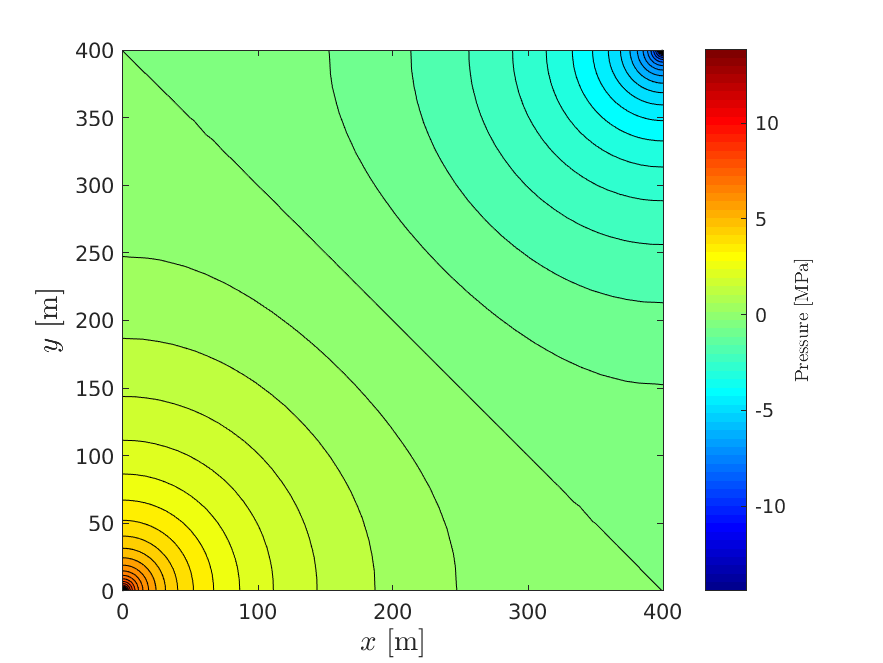
\includegraphics[width=1.0\textwidth]{./Figures/Examples/FiveSpot/5puntos2sol_2}
%		\caption[Test geometry 1]{Simulated pressure contours ($\mathrm{MPa}$).}
%		\label{fig:5puntos2}
%	\end{subfigure}\quad
%	\begin{subfigure}[b]{0.5\textwidth}
%	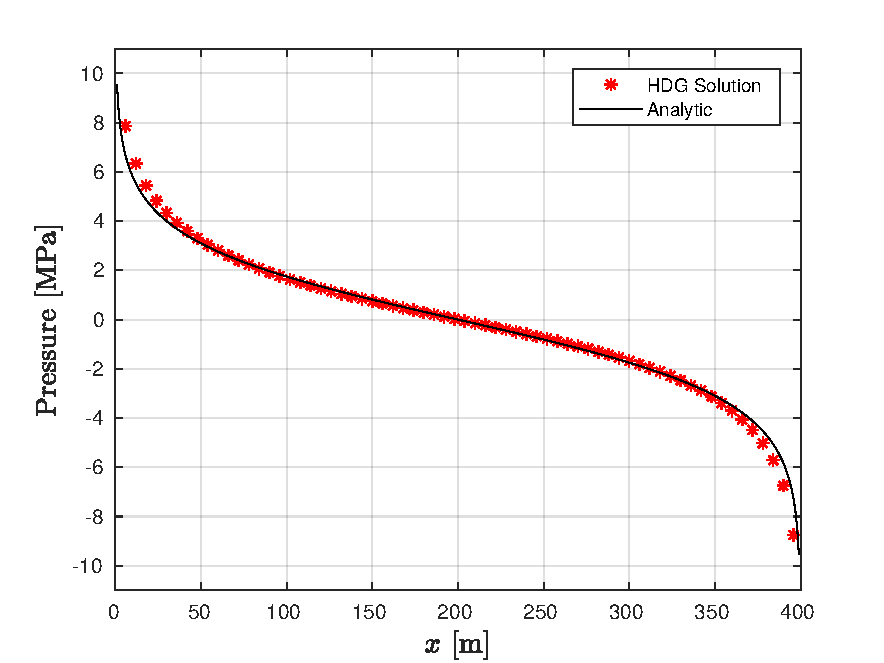
\includegraphics[width=1\textwidth]{./Figures/Examples/FiveSpot/5spot1_Diagonal.pdf}
%	\caption[Test geometry 1]{Pressure along the digonal ($\mathrm{MPa}$).}
%	\label{fig:5puntos1_Diag}
%	\end{subfigure}
%	\begin{subfigure}[b]{0.5\textwidth}
%		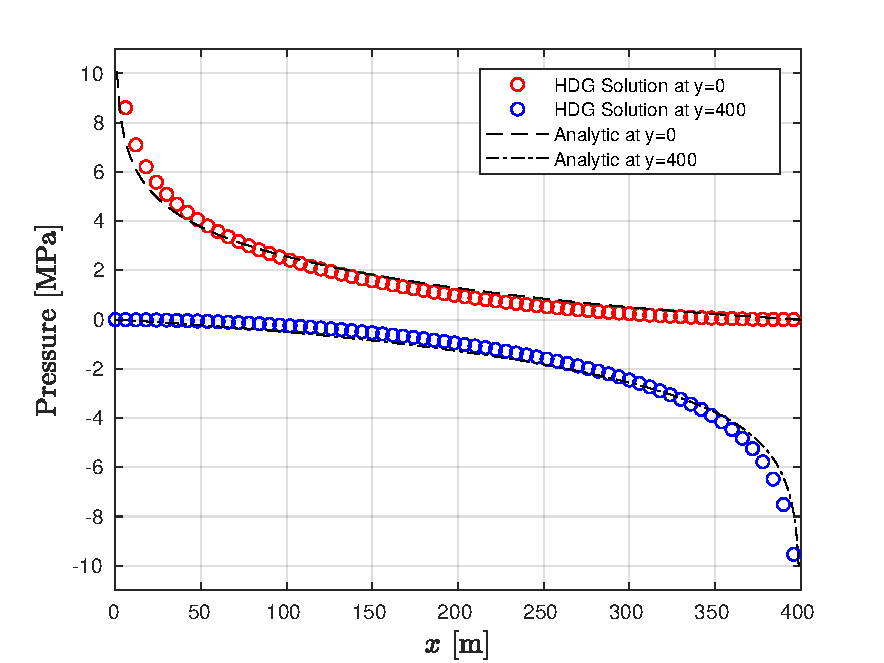
\includegraphics[width=\textwidth]{./Figures/Examples/FiveSpot/5spot1_BoundSol.pdf}
%		\caption[Test geometry 1]{Pressure along the $y$-boundaries. ($\mathrm{MPa}$).}
%		\label{fig:5puntos1_boundSol}
%	\end{subfigure}\quad
%    \begin{subfigure}[b]{0.5\textwidth}
%		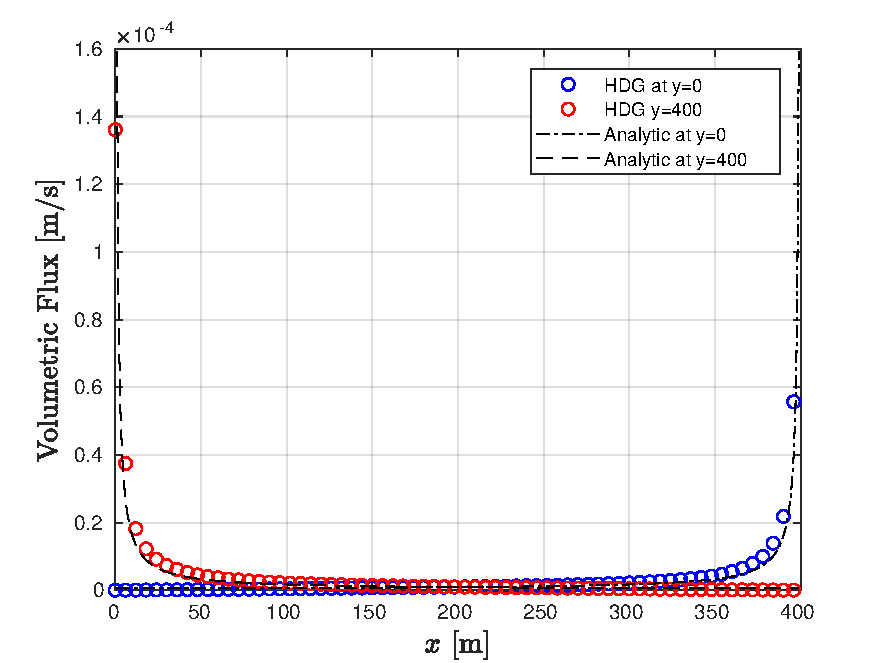
\includegraphics[width=\textwidth]{./Figures/Examples/FiveSpot/5spot1_BoundGrad.pdf}
%		\caption[Test geometry 1]{Volumetric flux along the $y$-boundaries ($\mathrm{m}/\mathrm{s}$).}
%		\label{fig:5puntos1_limit}
%	\end{subfigure}
%	\caption{Numerical results of the five-spot problem simulation.}
%	\label{fig:fiveResults}
%\end{figure}
%
%
%
%\begin{figure}[H]
%		\centering
%		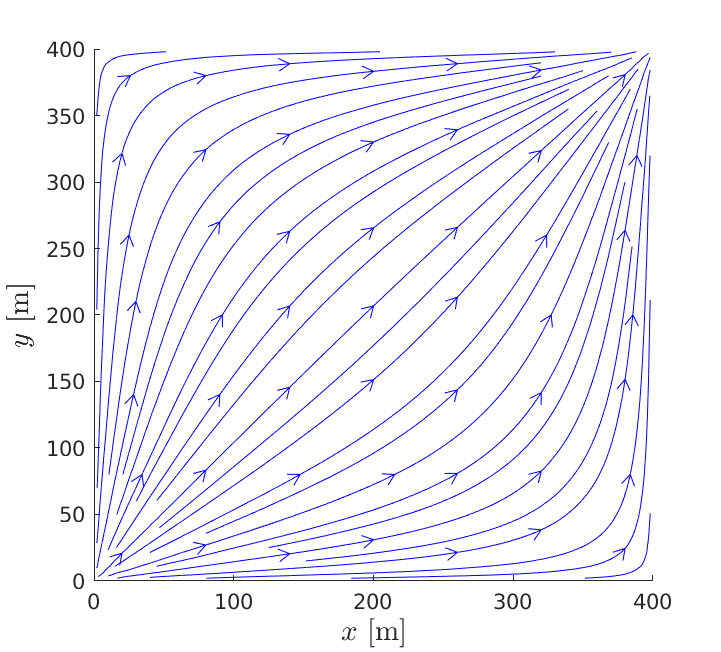
\includegraphics[width=0.6\textwidth]{./Figures/Examples/FiveSpot/5puntos2stream_2.pdf}
%		\caption[Test geometry 1]{Streamlines of the five spot problem.}
%		\label{fig:5puntos2stream1}
%\end{figure}
%
%
% The streamlines plot of the five-spot problem is presented in Figure \ref{fig:5puntos2stream1}. This results indicate that the fluid particles will travel from the injector well to the producer well, through the whole domain. \\
%
%
%Finally, the convergence of the relative error is presented in Table \ref{error5spot}., in terms of the number elements and degrees of freedom (dof), and mesh size $h$ (maximum element measure), for four different meshes. The error computation is done taking account of the analytical solution presented in equation \eqref{exact_5spot} and using the $L^2$ norm.
%
%\begin{table}[H]
%	\begin{center}
%		\begin{tabular}{|c||c|c|c|}
%			\hline
%			nElement & d.o.f  & $h$ [m] & Error \\ \hline\hline
%			 102     & 918    & 197.01  & 0.1632\\
%			 550     & 4950   & 115.04  & 0.0450\\ 	
%			 4282    & 38538  & 37.75   & 0.0245\\
%			 50020   & 450180 & 12.19   & 0.0125
%	 		\\ 
%			
%			\hline	
%		\end{tabular}
%		\caption{Convergence of the error with the $L^2$-norm.}\label{error5spot}
%	\end{center}
%\end{table}
%
%As it was expected, the error analysis presented in Table \ref{error5spot} indicates that the HDG  numerical solution converges to the analytical solution when the mesh is refined.
%
%\subsubsection{Case 2.}
%
%One of the most important and complex problems in the reservoir simulation is related to the fluid flow in fractured porous media \cite{sahimi2011flow}. The classical continuous models of the fractured systems, such as double permeability - double porosity models \cite{fractureGhafouri96,fractureLewis97,fractureHuyakorn83}, can not account for the fracture geometry and its interaction with other fractures in the reservoir. A discrete representation of the fracture network systems permits the study of such variables in a reservoir. However, more complexity to the computational grid is added because of the number of elements increases as well as the media heterogeneity.  In this case, the traditional methods must be adapted to search heterogeneity interfaces and in most cases, treat the interface as an internal boundary condition \cite{bobaru2012}.\\
%Due to the discontinuous nature of the approximation functions $(\unn_h,P_h)$ of HDG formulation, no additional search is required for heterogeneity boundaries, it is enough to set different values of the permeability function $\mathbb{K}(x,y)$ at the neighbor elements in heterogeneity interfaces. Now, to test the versatility of the method, in this case, we will create a highly heterogeneous domain by placing a ultra-low permeability barrier in the center of the domain having a permeability tensor magnitude much lower than the one of flow domain as was done in \cite{KATIYAR}. Therefore, in this problem, we face a permeability that is not continuous in space. The physical domain of this problem is displayed in the Figure \ref{fig:5puntos1ex2}.    
%
%\begin{figure}[H]
%	\centering
%	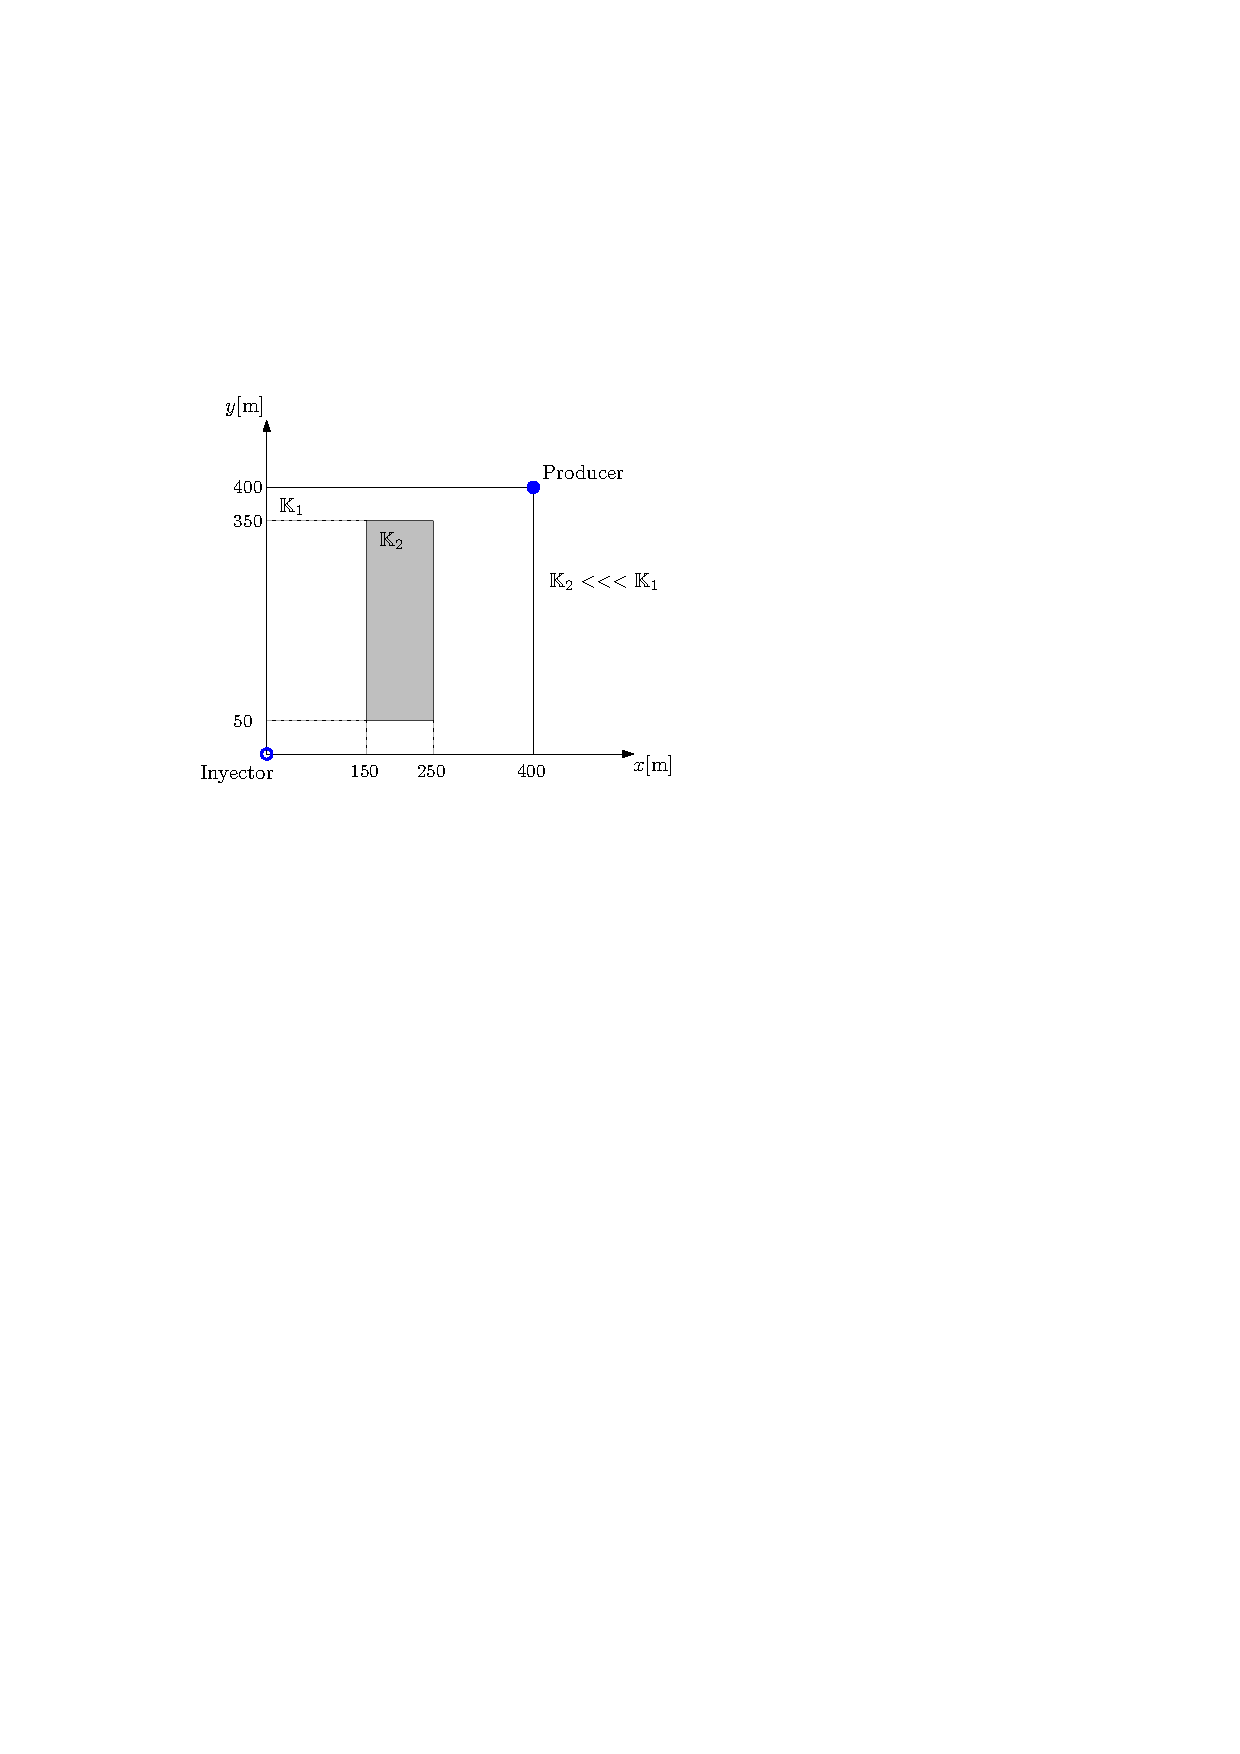
\includegraphics[width=0.6\linewidth]{./Figures/Examples/FiveSpot_Hetero/impermeable}
%	\caption[Test geometry 1]{Five-spot problem domain having a low-permeability barrier in the center.}
%	\label{fig:5puntos1ex2}
%\end{figure}
%Note that the permeability inside the barrier is not set to zero like in \cite{KATIYAR}, in order not to impose a discontinuous solution of an algorithmic type in the method, \textit{i.e.} modify the implementation to set the trivial solution to the equation \eqref{globalsis1}. In addition, this condition allows distribution of pressures inside the barrier, maintaining the continuity of the field of pressures throughout the domain. This is particularly useful in various fields of application such as, for example, reservoir geomechanics, where it is important to study the deformations of the porous medium due to the stresses produced by fluid flow.
%
%For this case, we consider the same units and flow features that we used in the previous examples, but having the following permeabilities for the domain and the barrier respectively:
%
%\begin{equation}
%\mathbb{K}_1 = \left[\begin{array}{cc}
%10^{-6} \, \mathrm{m^2} & 0 \\
%0 & 10^{-6} \, \mathrm{m^2}
%\end{array} \right] \qquad \text{and} \qquad \mathbb{K}_2 = \left[\begin{array}{cc}
%10^{-16} \, \mathrm{m^2} & 0 \\
%0 & 10^{-16} \, \mathrm{m^2}
%\end{array} \right].
%\end{equation}
%
%The numerical solution is presented in the Figures \ref{fig:fiveResult2} and \ref{fig:grad}.
%
%
%
%
%
%
%
%
%
%
%
%
%
%\begin{figure}[H]
%	\centering
%	\begin{subfigure}[b]{0.45\textwidth}
%		\centering
%		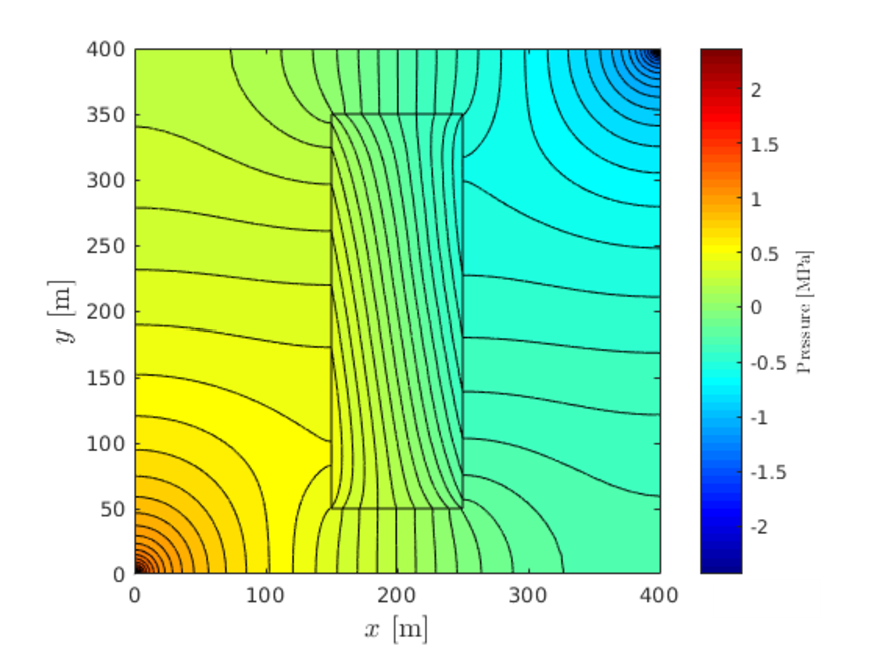
\includegraphics[width=\textwidth]{./Figures/Examples/FiveSpot_Hetero/contourHetero.pdf}
%		\caption[Test geometry 2]{Simulated pressure contours ($\mathrm{MPa}$).}
%		\label{fig:5puntosAni}
%	\end{subfigure}
%	\begin{subfigure}[b]{0.45\textwidth}
%		\centering
%		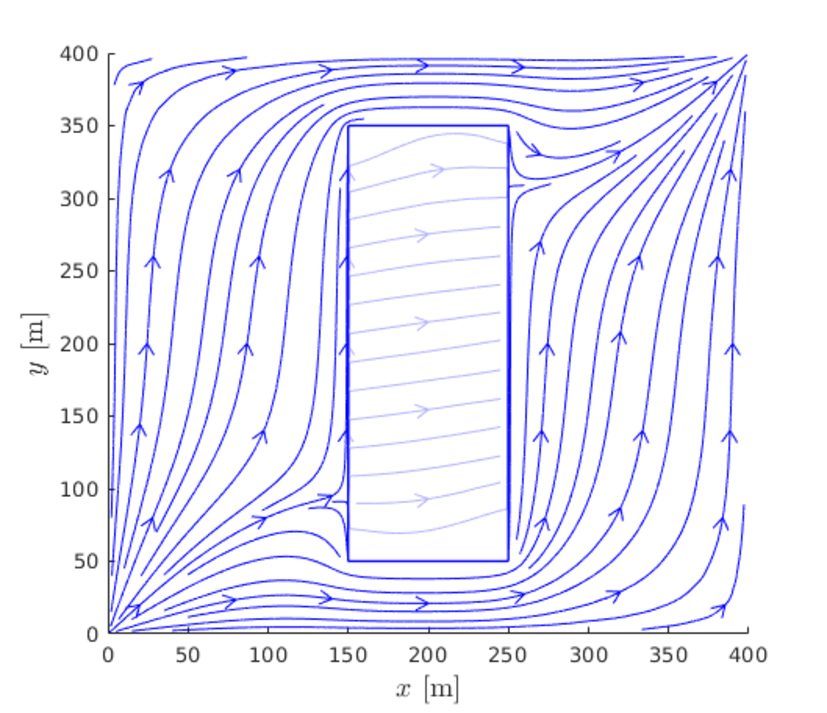
\includegraphics[width=0.85\textwidth]{./Figures/Examples/FiveSpot_Hetero/StreamlinesHetero.pdf}
%		\caption[Test geometry 2]{Streamlines of the numerical solution.}
%		\label{fig:5puntosAnistream}
%	\end{subfigure}
%
%	\begin{subfigure}[b]{0.45\textwidth}
%		\centering
%		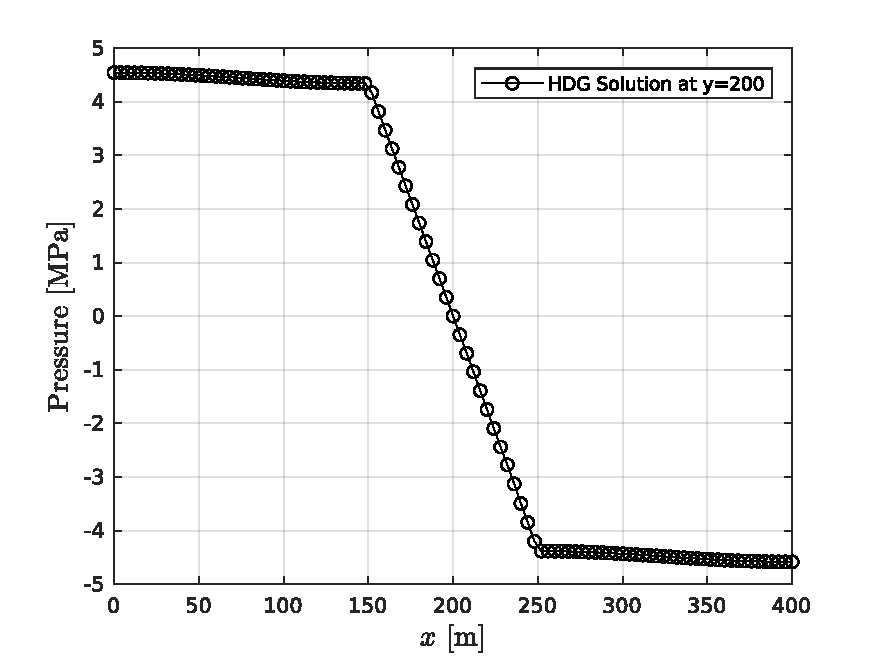
\includegraphics[width=\textwidth]{./Figures/Examples/FiveSpot_Hetero/5spot2_P_L200.pdf}
%		\caption[Test geometry 2]{Contour of the numerical solution pressure.}
%		\label{fig:5puntosAn2i}
%	\end{subfigure}
%	\begin{subfigure}[b]{0.45\textwidth}
%		\centering
%		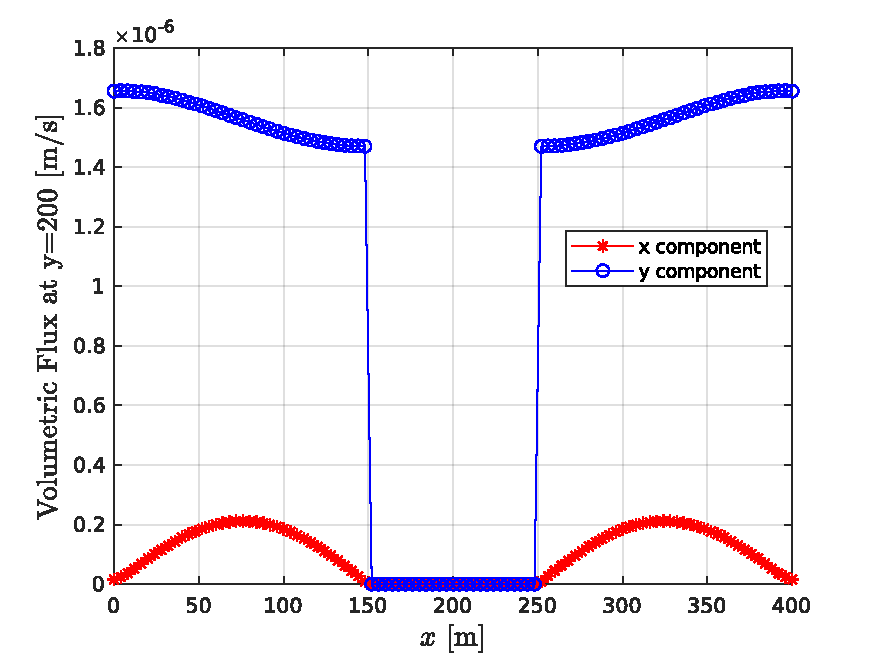
\includegraphics[width=1\textwidth]{./Figures/Examples/FiveSpot_Hetero/5spot2_Grad_L200}
%		\caption[Test geometry 2]{Volumetric flux components at $y=200$ ($\mathrm{m}/\mathrm{s}$).}
%		\label{fig:5puntos2_GradL200}
%	\end{subfigure}
%
%	\caption{Numerical solution in the heterogeneous case with $43136$ elements.}
%	\label{fig:fiveResult2}
%\end{figure}
%
%One important result is that, despite the pressure field it is continuous (Figure \ref{fig:5puntosAni}), the discontinuous permeability tensor field creates a discontinuous velocity filed, as observed at the interface of the barrier in the Figure \ref{fig:5puntos2_GradL200}.  Flow will proceed through preferential areas (high permeability zones) as the streamlines indicate in the Figure \ref{fig:5puntosAnistream}. Additionally, the Figure \ref{fig:grad} shows the magnitude of the gradient obtained directly as a result of the method. In this figure is evident the discontinuous nature of the HDG method, element by element, particularly in the jump of the velocity solution due to the abrupt change of the material in the faces of the barrier.
%
%
%\begin{figure}[H]
%	\centering
%	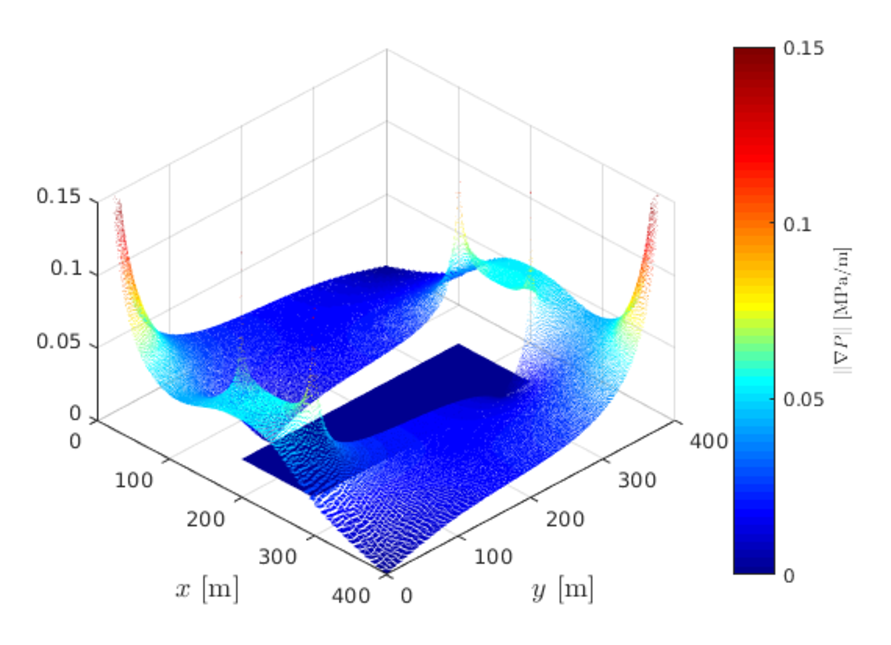
\includegraphics[width=0.6\linewidth]{./Figures/Examples/FiveSpot_Hetero/disc_Grad}
%	\caption[Test geometry 1]{Pressure gradient magnitude for the five-spot problem in heterogeneous case ($\mathrm{MPa}/\mathrm{m}$).}
%	\label{fig:grad}
%\end{figure}
%
%
%By the Darcy equation and the equation \eqref{diff2}, there is a proportionality relationship between the magnitude of the pressure gradient and the magnitude of the flow velocity in the porous media. Note also that, except for the regions around the source and the sink, there is an increase in the gradient in the narrow zones between the barrier and the north and south boundaries, indicating a significant increase in velocity that coincides with the narrowing of the streamlines in the Figure \ref{fig:5puntosAnistream}. Also, it is important to note that, due to the very low permeability in the barrier, the flow velocity is almost zero in the portion of the domain occupied by that obstacle.
%
%
%\section{Conclusion}
%This work is the basis for the construction of more robust numerical methods to face major problems related to flow in highly anisotropic and heterogeneous porous media, as many applications in the oil industry. It seems convenient to use numerical methods based on variational formulations of porous media because this approach allows more efficient modeling of flow dynamics in media with very special characteristics as a naturally fractured media. In highly anisotropic media, the HDG method proves to be efficient and this gives an idea about other applications that can have taking advantage over the classic methods as FVM and FEM. \\
%
%As we show in the five spot problem with the barrier, HDG method takes advantage of the discontinuous nature of the solution, and his gradient (see Figure \ref{fig:grad}), in heterogeneous porous media where the permeability function is highly discontinuous in space. This property of the mixed methods is particularly useful to calculate the velocity fields of the solution in this kind of heterogeneous domains because the proportionality relation between the gradient and the velocity given by Darcy's law. Also, is important to note that the proposed HDG formulation can simulate such discontinuities without any extra assumption or additional computational expense as searching algorithms usually required for heterogeneity interfaces.
%Additionally, HDG has a fundamental advantage over the classical DG methods, which is the reduction of the degrees of freedom in the formulation, because the normal trace continuity weakly imposed in the solution. In addition, HDG for the mixed formulation possesses conservative properties, like FVM, with the inherited advantages of the finite element method.\\
%
%The next stage of this work is to analyze and to compare the performance of the HDG method here presented with respect to the classical methods as FVM and FEM. The current development and implementation of HDG are planned to be extended to more general diffusion problems involving time, three-dimensional domains and two face flow. 
%
%\section*{Acknowledgments}
%Authors thank Equion, COLCIENCIAS and the Agencia Nacional de Hidorcarburos for
%financial support under Contract No. 273-2017: \textit{Plan Nacional para el Potenciamiento de la Tecnolog\'{i}a CEOR con Gas
%	Mejorado Qu\'{i}micamente}. Authors also thank Universidad Nacional de Colombia for logistic and financial support.
%
%
%\bibliography{biblio1}

\end{document}